\documentclass[UTF8,AutoFakeBold]{ctexart}
\usepackage[a4paper,left=2.5cm,right=2.5cm,top=3cm,bottom=2.5cm]{geometry}
\usepackage{ctex}
\usepackage{float}
\usepackage{graphicx}
\usepackage{subfigure}
\usepackage{makecell}
\usepackage{listings}
\usepackage{fontspec}
\usepackage{amsmath}
\usepackage[dvipsnames]{xcolor}
\setmainfont{Times New Roman}
\usepackage[framed,numbered,autolinebreaks,useliterate]{mcode}
\lstset{language=Matlab,
		basicstyle=\normalsize,
		basicstyle=\small,
		numberstyle=\tiny,
		breaklines=true,
		extendedchars=false,
		columns=flexible,
		numbers=left,
		numbersep=2em,
		numberstyle=\footnotesize,
		frame=single,
		framesep=1em,
		xleftmargin=-2em}
\pagestyle{empty}
\begin{document}
	\begin{table}
		\begin{figure}[H]
			\centering
			\quad \\[50pt]
			
\includegraphics[width=9.98cm,scale=1.51]{./figures/ico.jpg}
			\quad \\[33.5pt]
		\end{figure}
	\end{table}
	\begin{center}
		\bfseries\heiti\zihao{0}《信号与系统》课程\\[14pt]
		实验报告
	\end{center}
%	\hspace*{\fill} \\[5pt]
	\quad \\*
	\begin{table}[H]
		\centering
		\begin{tabular}[top]{cc}
			\rule{0pt}{25pt}
			\makebox[7em][s]{\songti\zihao{-3}学\hspace{\fill}院}\  & \makebox[16em][s]{\songti\zihao{-3}信息科学与工程学院} \\
			\Xcline{2-2}{1.2pt}
			\rule{0pt}{25pt}
			
			\makebox[7em][s]{\songti\zihao{-3}专\hspace{\fill}业}\  & \makebox[16em][s]{\songti\zihao{-3}电子信息科学与技术} \\
			\Xcline{2-2}{1.2pt}
			\rule{0pt}{25pt}
			
			\makebox[7em][s]{\songti\zihao{-3}班\hspace{\fill}级}\  & {\zihao{-3}20\songti\zihao{-3}阳明2班} \\
			\Xcline{2-2}{1.2pt}
			\rule{0pt}{25pt}
			
			\makebox[7em][s]{\songti\zihao{-3}学\hspace{\fill}号}\  & {\zihao{-3}206001232} \\
			\Xcline{2-2}{1.2pt}
			\rule{0pt}{25pt}
			
			\makebox[7em][s]{\songti\zihao{-3}姓\hspace{\fill}名}\  & {\songti\zihao{-3}熊\quad \songti\zihao{-3}康} \\
			\Xcline{2-2}{1.2pt}
			\rule{0pt}{25pt}
			
			\makebox[7em][s]{\songti\zihao{-3}指导教师}\  & {\songti\zihao{-3}李\quad \songti\zihao{-3}军} \\
			\Xcline{2-2}{1.2pt}
			\rule{0pt}{41.6pt}
			
			\makebox[7em][s]{\songti\zihao{-3}完成日期}\  & {\songti\zihao{-3}2022\songti\zihao{-3}年3\songti\zihao{-3}月30\songti\zihao{-3}日} \\
			\Xcline{2-2}{1.2pt}
		\end{tabular}
	\end{table}
	\newpage
	\begin{center}
		{\bfseries\heiti\zihao{-2}实验二\quad 连续和离散时间LTI系统的响应及卷积}
	\end{center}
	\setcounter{section}{1}
	\subsection{{\heiti\zihao{4}实验目的}}
	\begin{enumerate}
		\item [(1)] 掌握有关信号时域的测量方法;
		\item [(2)] 利用 Matlab 工具箱求解连续时间系统的冲激响应、阶跃响应,离散时间系统的单位样值响应,理解卷积概念。
	\end{enumerate}
	\subsection{{\heiti\zihao{4}实验原理(或实验方法)}}
	\subsubsection{{\heiti\zihao{5}卷积的含义}}
		卷积积分的物理意义是将信号分解为冲激信号之和,借助系统的冲激响应,求解系统对任意激励信号的零状态响应。设系统的激励信号为
		$x(t)$ ,冲激响应为 $h(t)$ ,则系统的零状态响应为
		\begin{align}
		y(t)=x(t)*h(t)= \int_{-\infty}^{+\infty}x(t)h(t-\tau )d\tau
		\end{align}\par
		对于任意两个信号$f_1(t)$和$f_2(t)$,两者做卷积运算定义为:
		\begin{equation}
		f(t)=\int_{-\infty}^{+\infty}f_1(t)f_2(t-\tau)d\tau=f_1(t)*f_2(t)=f_2(t)*f_1(t)
		\end{equation}\par

	\subsubsection{\heiti\zihao{5}两个矩形脉冲信号的卷积过程}
		两信号$x(t)$ 与 $h(t)$ 都为矩形脉冲信号,图1 用由图解的方法给出了两个信号的卷积过程和结
	果,可以与实验结果进行比较。
		\begin{figure}[ht]
			\centering
			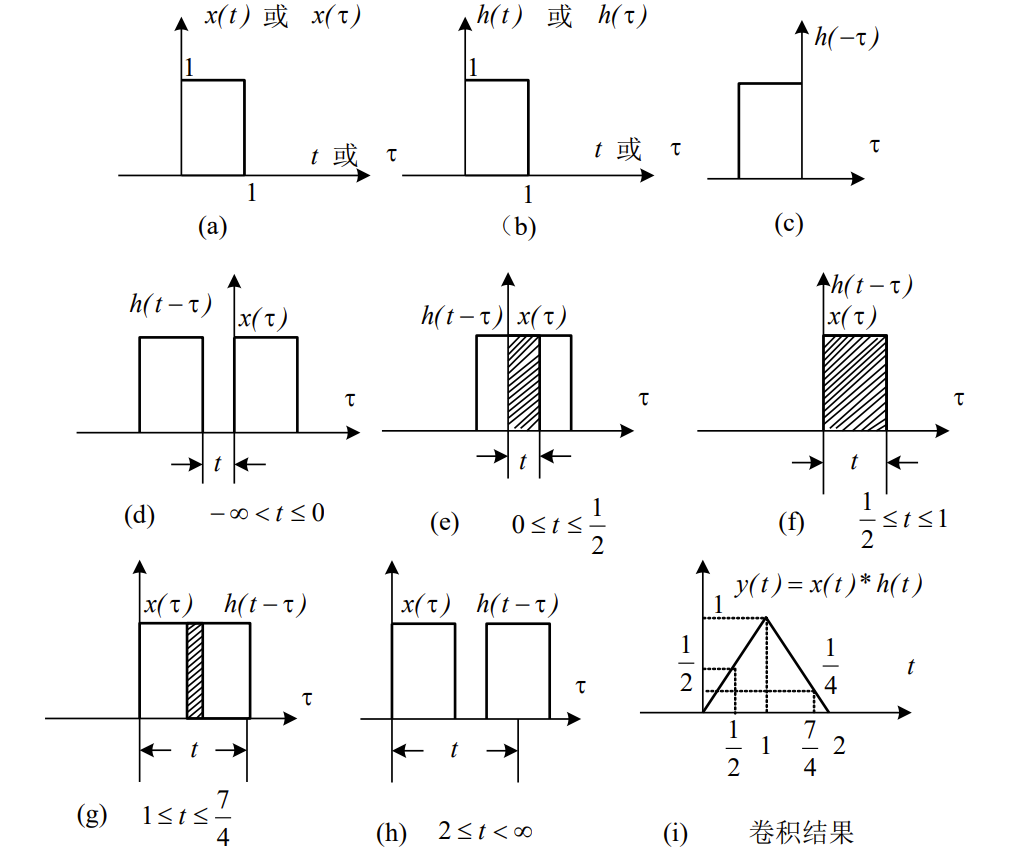
\includegraphics[scale=0.4]{./figures/photo1.png}
			\caption{两矩形脉冲的卷积积分的运算过程与结果}
		\end{figure}

	\subsubsection{\heiti\zihao{5}矩形脉冲信号与锯齿波信号的卷积}
	信号$f_1(t)$为矩形脉冲信号,$f_2(t)$ 为锯齿波信号,如图 2 所示。根据卷积积分的运算方法得到$f_1(t)$ 和$f_2(t)$ 的卷积积分结果$f_(t)$,如图 2(c)所示。
		\begin{figure}[ht]
			\centering
			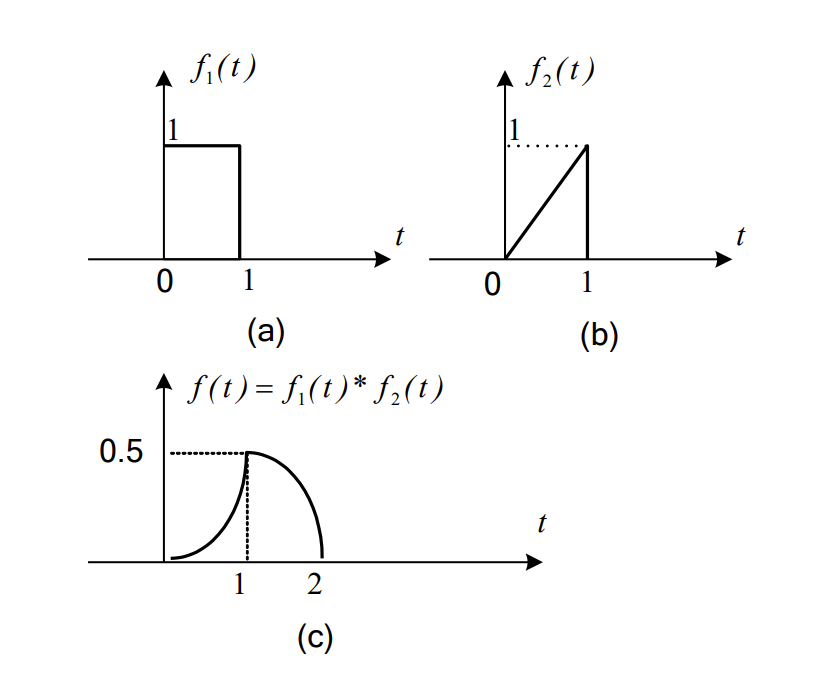
\includegraphics[scale=0.5]{./figures/photo2.png}
			\caption{矩形脉冲信号与锯齿脉冲信号的卷积积分的结果}
		\end{figure}




	\subsection{{\heiti\zihao{4}实验内容}}
%		源程序(要有,附上必要的注释)\\
%		实验结果(图形)(图形大小、位置适中)\\
%		结果说明或分析
	\begin{enumerate}
		\item[(1)] 连续时间系统的冲击响应、阶跃响应
		\begin{enumerate}
			\item[(a)] 利用 impulse 函数画出教材 P43 例 2-17: LTI 系统\par
				$\frac{d^2 y(t)}{d t^2}+4\frac{dy(t)}{dt}+3y(t)=\frac{dx(t)}{dt}-x(t)$的冲击响应的波形。
			
%	插入代码需要靠到最左边
		\begin{lstlisting} 
%%%%%%%%%%%%%%%%%%%%%%%%%%%%%%%%%%%%%%%%%%%%%%% 
% Author:  熊康
% E-mail: 206001232@nbu.edu.cn
% Tool:    MATLAB R2018b
% Function:利用impulse函数画出LTI系统冲激响应的波形
% Version: 2022-3-23 v1.0
%%%%%%%%%%%%%%%%%%%%%%%%%%%%%%%%%%%%%%%%%%%%%%%

clear;clc;
sys = tf([1, -1],[1, 4, 3]);
figure('Color', 'White', 'Position', [100 100 640 240], 'MenuBar', 'None');
impulse(sys);
t = 0: 0.1: 6;
y = (2.*exp(-3*t)-exp(-t)).*(t>=0);
hold on
plot(t, y);

axis([-0.1, 6.1, -0.8, 1.1]);
set(gca, 'FontName', 'Times New Roman', 'FontSize', 10, 'LineWidth', 2);
set(gca, 'XTick', -0 : 1 : 6);
set(gca, 'YTick', -0.5 : 0.2 : 1);

xlabel('Time \itt\rm');
ylabel('\itg\rm(\itt\rm)');
legend('Function Solve','Equation Solve');
		\end{lstlisting}

		\begin{figure}[H]
			\centering
			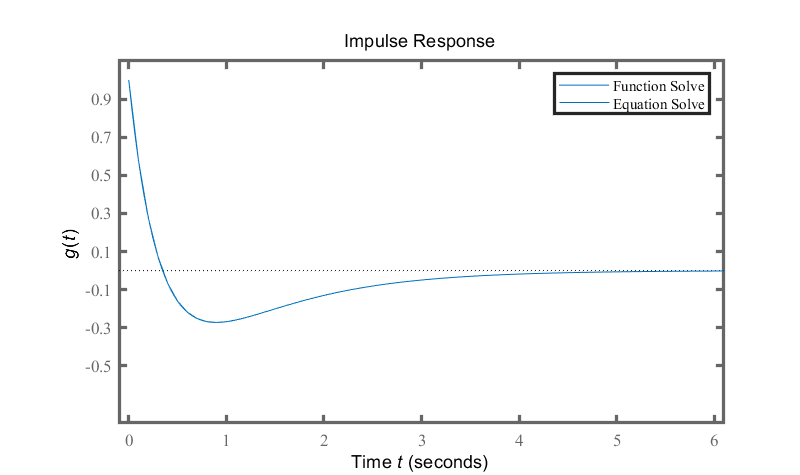
\includegraphics[scale=0.6]{./figures/photo3.png}
			\caption{冲击响应的波形}
		\end{figure}
		\textbf{\songti 分析:}由图可知,MATLAB的impulse函数求得的解和通过方程求得的解基本一致。系统响应$g(t)$从1快速递减至-0.3,然后缓慢递增并趋向于0。 

			\item[(b)] 利用 step 函数画出教材 P44 例 2-18: LTI 系统\par
				$y^{n} (t)+3y^{'} (t)+2y(t)=3x^{'}(t)+2x(t)$的阶跃响应的波形。
				\begin{lstlisting}
%%%%%%%%%%%%%%%%%%%%%%%%%%%%%%%%%%%%%%%%%%%%%%% 
%Author:  熊康
%E-mail: 206001232@nbu.edu.cn
%Tool:    MATLAB R2018b
%Function:利用step函数画出LTI系统的阶跃响应的波形
%Version: 2022-3-23 v1.0
%%%%%%%%%%%%%%%%%%%%%%%%%%%%%%%%%%%%%%%%%%%%%%%

clear;clc;
D_c = [1 3 2];
N_c = [3 2];
figure('Color', 'White', 'Position', [100 100 640 380]');
step(N_c, D_c);
t = 0: 0.1: 6;
y = ((-2).*exp(-2*t)+exp(-t)+1).*(t>=0);
hold on 
plot(t, y)
axis([-0.1, 6.1, -0.1, 1.3]);
set(gca, 'FontName', 'Times New Roman', 'FontSize', 10, 'LineWidth', 2);
set(gca, 'XTick', -0 : 1 : 6);
set(gca, 'YTick', -0 : 0.2 : 1.4);
xlabel('Time \itt\rm');
ylabel('\itg\rm(\itt\rm)');
title('Step response');
legend('Function Solve','Equation Solve');
				\end{lstlisting}
				\begin{figure}[H]
					\centering
					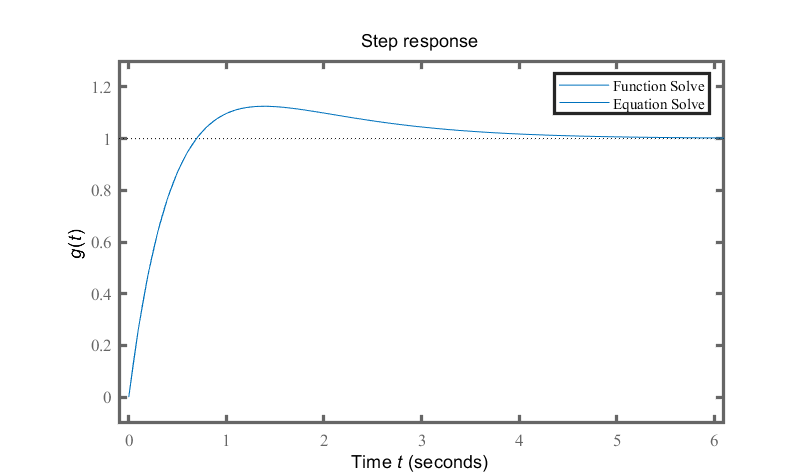
\includegraphics[scale=0.6]{./figures/photo4.png}
					\caption{阶跃响应的波形}
				\end{figure}
			
				\textbf{\songti 分析:} 由图可知,MATLAB的step函数求得的解和通过方程求得的解基本一致。系统响应$g(t)$从0快速递增至1.1,然后缓慢递减并趋向于1。 
		\end{enumerate}

		
		\begin{enumerate}
			\item[(2)] 离散时间系统的单位样值响应\par
			利用impz函数画出教材P47例2-22:\par
			$y[n]-3y[n-1]+3y[n-2]-y[n-3]=x[n]$的单位样值相应的图形。
		
			\begin{lstlisting}
%%%%%%%%%%%%%%%%%%%%%%%%%%%%%%%%%%%%%%%%%%%%%%% 
%Author:  熊康
%E-mail: 206001232@nbu.edu.cn
%Tool:    MATLAB R2018b
%Function:利用impz函数画出单位样值响应的图形
%Version: 2022-3-23 v1.0
%%%%%%%%%%%%%%%%%%%%%%%%%%%%%%%%%%%%%%%%%%%%%%%

clear;clc;
D_c = [1 -3 3 -1];
N_c = 1;

figure('Color', 'White', 'Position', [100 100 640 240]);
impz(N_c, D_c);
axis([-1, 10, 0, 60]);
set(gca, 'FontName', 'Times New Roman', 'FontSize', 10, 'LineWidth', 2);
% set(gca, 'XTick', -0 : 1 : 6);
% set(gca, 'YTick', -0 : 0.2 : 1.4);

n = 0: 1: 9;
y = n.^2 /2 + 3.*n /2 + 1;
hold on
plot(n, y, '*');
xlabel('Time \itt\rm');
ylabel('\itg\rm(\itt\rm)');
legend('Function Solve','Equation Solve');
				\end{lstlisting}
				\begin{figure}[H]
					\centering
					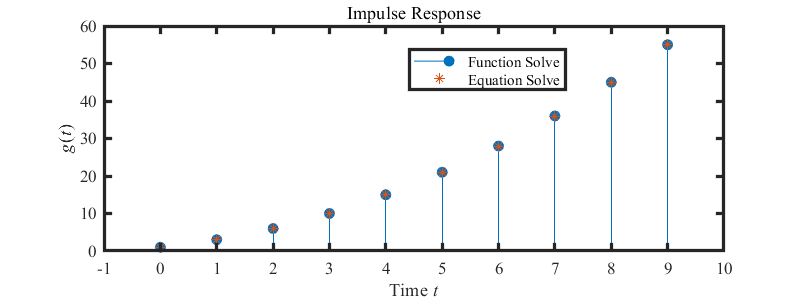
\includegraphics[scale=0.6]{./figures/photo5.png}
					\caption{离散时间系统的单位样值响应的图形}
				\end{figure}

				\textbf{\songti 分析:} 由图可知,MATLAB的impz函数求得的解和通过方程求得的解基本一致。系统响应$g(t)$从1开始递增,递增速度随时间变快。
		\end{enumerate}


		\begin{enumerate}
			\item[(3)] 画出函数 $f_1(t)=(1+t)[u(t)-u(t-1)]$和 $f_2(t)=u(t-1)-u(t-2)$的图形,并利用附在后面的 sconv.m 函
			数画出卷积积分 $f_1(t)* f_2(t)$图形。
		
			\begin{lstlisting}
%%%%%%%%%%%%%%%%%%%%%%%%%%%%%%%%%%%%%%%%%%%%%%% 
%Author:  熊康
%E-mail: 206001232@nbu.edu.cn
%Tool:    MATLAB R2018b
%Function:画出卷积积分 f1(t)* f2(t)图形
%Version: 2022-3-23 v1.0
%%%%%%%%%%%%%%%%%%%%%%%%%%%%%%%%%%%%%%%%%%%%%%%

%function sconv
%计算连续信号卷积积分 f(t) = f1(t) * f2(t);
% f: 卷积积分 f(t)对应的非零样值向量;
% f_1_t : f1(t)非零样值向量;
% f_2_t : f2(t)的非零样值向量;
% t1 : f1(t)的对应时间向量;
% t2 : f2(t)的对应时间向量;
% t_conv:f(t)的对应时间向量;
% dt:取样时间间隔;

dt = 0.01;
t1 = 0 : dt : 1;
t2 = 1 : dt : 2;
f_1_t = 1 + t1;
f_2_t = t2 .* 0 + 1;
	
sconv(f_1_t, f_2_t, t1, t2, dt);

t = 1: 0.1: 3;
y = (t.^2 /2 - 0.5).*(t>=1) + (-t.^2 + t + 2).*(t>=2) + (t.^2/2 - t - 1.5).*(t>=3);
hold on
plot(t, y ,'*');
legend('Function Solve','Equation Solve');
				\end{lstlisting}

				\begin{lstlisting}
%%%%%%%%%%%%%%%%%%%%%%%%%%%%%%%%%%%%%%%%%%%%%%% 
%Author:  熊康
%E-mail: 206001232@nbu.edu.cn
%Tool:    MATLAB R2018b
%Function:函数sconv画出卷积积分 f1(t)* f2(t)图形
%Version: 2022-3-23 v1.0
%%%%%%%%%%%%%%%%%%%%%%%%%%%%%%%%%%%%%%%%%%%%%%%

function [f, t_conv] = sconv(f_1_t, f_2_t, t1, t2, dt)
%计算连续信号卷积积分 f(t) = f1(t) * f2(t);
% f: 卷积积分 f(t)对应的非零样值向量;
% f_1_t : f1(t)非零样值向量;
% f_2_t : f2(t)的非零样值向量;
% t1 : f1(t)的对应时间向量;
% t2 : f2(t)的对应时间向量;
% t_conv:f(t)的对应时间向量;
% dt:取样时间间隔;
f = conv(f_1_t, f_2_t); %计算序列 f1 与 f2 的卷积和 f;
f = f * dt;
t_start = t1(1) + t2(1); %计算序列 f 非零样值的起点位置;
n_count = length(f_1_t) + length(f_2_t)- 2; %计算卷积和 f 的非零样值的宽度;
t_end = t_start + n_count * dt;
t_conv = t_start : dt : t_end; %卷积和 f 非零样值的时间向量;
figure('Color', 'White', 'Position', [100 100 960 480]);
subplot(2, 2, 1);
plot(t1, f_1_t, 'LineWidth', 2); %在子图 1 绘 f1(t)时域波形图;
axis([t1(1)-0.1, t1(1)+length(f_1_t)*dt+0.1, -0.1, 2.1]);
set(gca, 'FontName', 'Times New Roman', 'FontSize', 10, 'LineWidth', 2);
set(gca, 'XTick', t1(1) : 1 : t1(1)+length(f_1_t)*dt);
set(gca, 'YTick', 0 : 0.5 : 2);
xlabel('Time \itt\rm');
ylabel('\itf\rm_1(\itt\rm)');
% title('信号\itf\rm_1(\itt\rm)');
subplot(2, 2, 2);
plot(t2, f_2_t, 'LineWidth', 2); %在子图 2 绘 f2(t)时波形图;
axis([t2(1)-0.1, t2(1)+length(f_2_t)*dt+0.1, -0.1, 2.1]);
set(gca, 'FontName', 'Times New Roman', 'FontSize', 10, 'LineWidth', 2);
set(gca, 'XTick', t2(1) : 1 : t2(1)+length(f_2_t)*dt);
set(gca, 'YTick', 0 : 0.5 : 2);
xlabel('Time \itt\rm');
ylabel('\itf\rm_2(\itt\rm)');
% title('信号\itf\rm_2(\itt\rm)');
subplot(2, 2, [3, 4]);
plot(t_conv, f, 'LineWidth', 2); %画卷积 f(t)的时域波形;
set(gca, 'FontName', 'Times New Roman', 'FontSize', 10, 'LineWidth', 2);
axis([t_start - 0.1 t_end + 0.1 -0.1 2.1]);
set(gca, 'FontName', 'Times New Roman', 'FontSize', 10, 'LineWidth', 2);
set(gca, 'XTick', t_start : 1 : t_end);
set(gca, 'YTick', 0 : 0.5 : 2);
xlabel('Time \itt\rm');
ylabel('\itf\rm(\itt\rm)');
% title('实验 2-3 两信号的卷积积分 \itf\rm(\itt\rm)=\itf\rm_1(\itt\rm)*\itf\rm_2(\itt\rm)');
end
				\end{lstlisting}
				\begin{figure}[H]
					\centering
					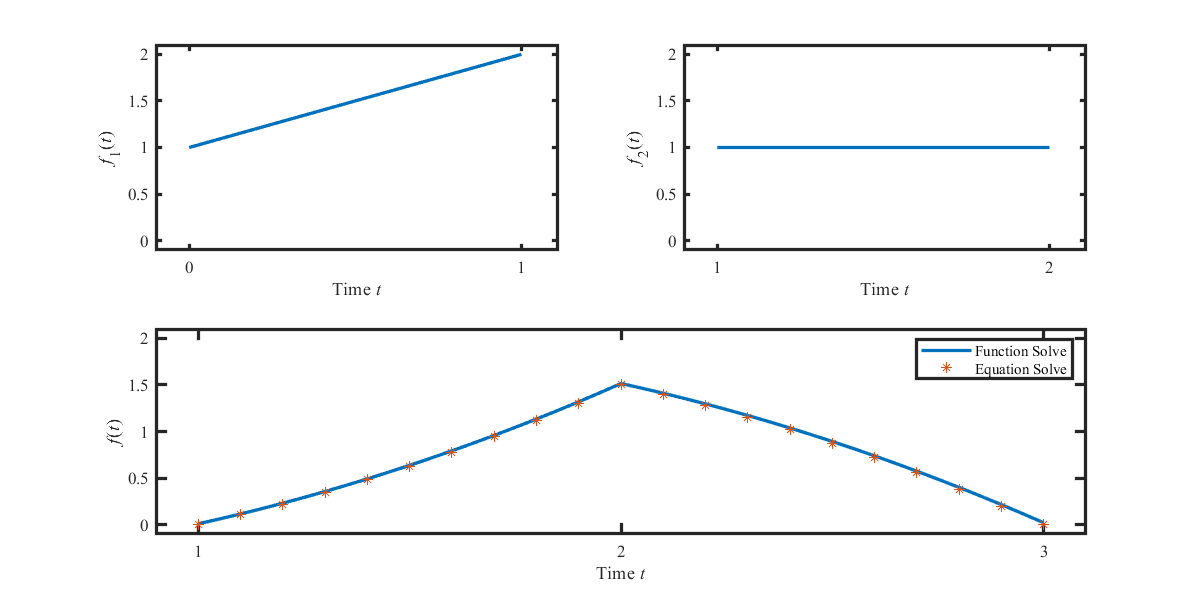
\includegraphics[scale=0.5]{./figures/photo6.png}
					\caption{卷积积分 $f_1(t)* f_2(t)$图形}
				\end{figure}

				\textbf{\songti 分析:} 左上角为$f_1(t)=(1+t)[u(t)-u(t-1)]$的图形,右上角为$f_2(t)=u(t-1)-u(t-2)$的图形,下面的是两者卷积积分后的图形。由图可知,通过MATLAB卷积公式求得的解和利用卷积性质求得的解基本一致。图形时域宽度为$t\in [1,3]$,从0快速递增,在$t=2$时刻$f(t)$递增至1.5,后又开始递减,并在$t=3$时刻$f(t)$递减至0。
		\end{enumerate}


		\begin{enumerate}
			\item[(4)] 画出教材 P58 例 2-30 中 $h[n]$、$x[n]$的图形(图 2-17(a)(b)),并利用 conv 函数求出卷积 $x[n]*h[n]$并画出图形(图 2-17(f))。	
			\begin{lstlisting}
%%%%%%%%%%%%%%%%%%%%%%%%%%%%%%%%%%%%%%%%%%%%%%% 
%Author:  熊康
%E-mail: 206001232@nbu.edu.cn
%Tool:    MATLAB R2018b
%Function:画出卷积和 x[n]*h[n] 图形
%Version: 2022-3-23 v1.0
%%%%%%%%%%%%%%%%%%%%%%%%%%%%%%%%%%%%%%%%%%%%%%%
clear;clc;

dt = 1;
t1 = [-1 0 1 2 3 4 5];
t2 = [-1 0 1 2 3 4 5];
f_1_t = [0 1 1 1 0 0 0];
f_2_t = [0 1 2 1 0 0 0];


nconv(f_1_t, f_2_t, t1, t2, dt);

t = 0 : 1 : 4;
y = [1 3 4 3 1];
hold on
plot(t, y ,'*');
legend('Function Solve','Equation Solve');
				\end{lstlisting}

				\begin{lstlisting}
%%%%%%%%%%%%%%%%%%%%%%%%%%%%%%%%%%%%%%%%%%%%%%% 
%Author:  熊康
%E-mail: 206001232@nbu.edu.cn
%Tool:    MATLAB R2018b
%Function:函数nconv画出卷积和 x[n]*h[n] 图形
%Version: 2022-3-23 v1.0
%%%%%%%%%%%%%%%%%%%%%%%%%%%%%%%%%%%%%%%%%%%%%%%

function [f, t_conv] = nconv(f_1_t, f_2_t, t1, t2, dt)
%计算连续信号卷积积分 f(t) = f1(t) * f2(t);
% f: 卷积和 f(t)对应的非零样值向量;
% f_1_t : f1(t)非零样值向量;
% f_2_t : f2(t)的非零样值向量;
% t1 : f1(t)的对应时间向量;
% t2 : f2(t)的对应时间向量;
% t_conv:f(t)的对应时间向量;
% dt:取样时间间隔;


f = conv(f_1_t, f_2_t); %计算序列 f1 与 f2 的卷积和 f;
f = f * dt;
t_start = t1(1) + t2(1); %计算序列 f 非零样值的起点位置;
n_count = length(f_1_t) + length(f_2_t)- 2; %计算卷积和 f 的非零样值的宽度;
t_end = t_start + n_count * dt;
t_conv = t_start : dt : t_end; %卷积和 f 非零样值的时间向量;
figure('Color', 'White', 'Position', [100 100 960 480]);
subplot(2, 2, 1);
plot(t1, f_1_t, 'o', 'LineWidth', 2); %在子图 1 绘 f1(t)时域波形图;
% axis([t1(1)-0.1, t1(1)+length(f_1_t)*dt+0.1, -0.1, 2.1]);
set(gca, 'FontName', 'Times New Roman', 'FontSize', 10, 'LineWidth', 2);
set(gca, 'XTick', t1(1) : 1 : t1(1)+length(f_1_t)*dt);
set(gca, 'YTick', 0 : 0.5 : 2);
xlabel('Time \itt\rm');
ylabel('\itf\rm_1(\itt\rm)');
% title('信号\itf\rm_1(\itt\rm)');
subplot(2, 2, 2);
plot(t2, f_2_t, 'o','LineWidth', 2); %在子图 2 绘 f2(t)时波形图;
% axis([t2(1)-0.1, t2(1)+length(f_2_t)*dt+0.1, -0.1, 2.1]);
set(gca, 'FontName', 'Times New Roman', 'FontSize', 10, 'LineWidth', 2);
set(gca, 'XTick', t2(1) : 1 : t2(1)+length(f_2_t)*dt);
set(gca, 'YTick', 0 : 0.5 : 2);
xlabel('Time \itt\rm');
ylabel('\itf\rm_2(\itt\rm)');
% title('信号\itf\rm_2(\itt\rm)');
subplot(2, 2, [3, 4]);
plot(t_conv, f,  'o','LineWidth', 2); %画卷积 f(t)的时域波形;
set(gca, 'FontName', 'Times New Roman', 'FontSize', 10, 'LineWidth', 2);
% axis([t_start - 0.1 t_end + 0.1 -0.1 2.1]);
set(gca, 'FontName', 'Times New Roman', 'FontSize', 10, 'LineWidth', 2);
set(gca, 'XTick', t_start : 1 : t_end);
set(gca, 'YTick', 0 : 0.5 : 2);
% xlabel('Time \itt\rm');
ylabel('\itf\rm(\itt\rm)');
end
				\end{lstlisting}	
				\begin{figure}[H]
					\centering
					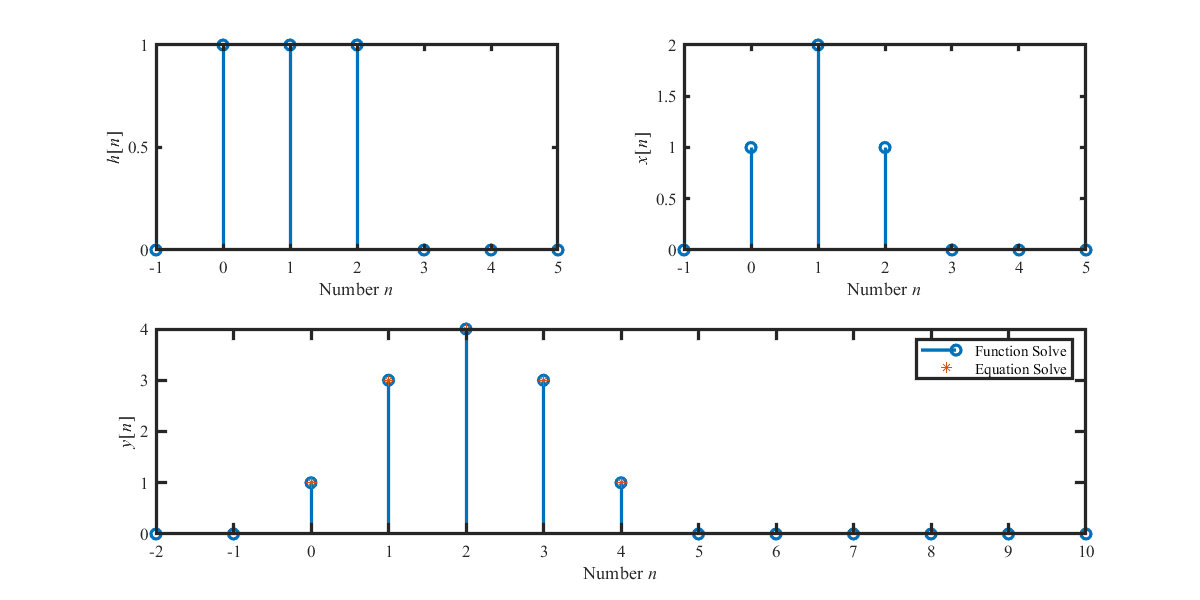
\includegraphics[scale=0.5]{./figures/photo7.png}
					\caption{卷积和$x[n]*h[n]$的图形}
				\end{figure}

				\textbf{\songti 分析:} 左上角为序列$h[n]$的图形,右上角为$x[n]$的图形,下面的是两者卷积和$y[n]=x[n]*h[n]$后的图形。由图可知,通过MATLAB卷积公式求得的解和利用卷积性质求得的解基本一致。图形宽度为$n\in [-2,10]$,从-2到-1为0,从0开始递增,在$n=2$时$y[n]$递增至4,后又开始递减,并在$n=5$时$y[n]$递减至0,此后$y[n]=0$。
		\end{enumerate}
	\end{enumerate}

	\subsection{{\heiti\zihao{4}思考题}}
	\begin{enumerate}
		\item[(1)] 矩形脉冲信号的脉冲宽度为什么会对卷积结果有影响,影响是什么?
		\item[(2)] 用图解的方法给出下图 8 中的两个信号的卷积过程。
		\begin{figure}[H]
			\centering
			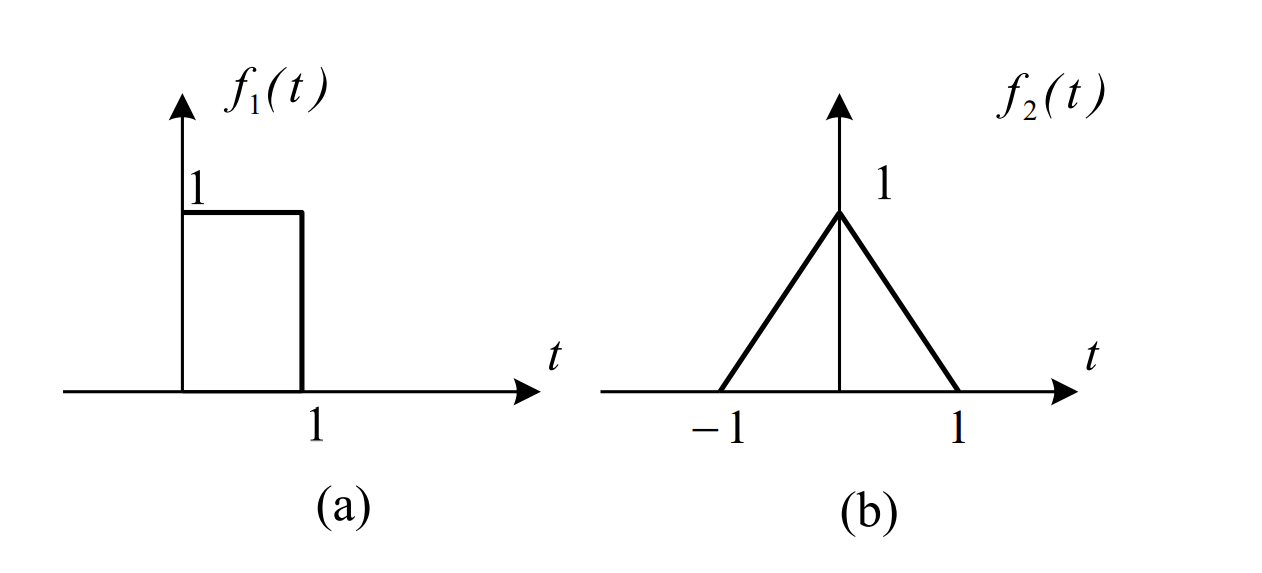
\includegraphics[scale=0.4]{./figures/photo8.png}
			\caption{矩形脉冲信号与三角波信号}
		\end{figure}
		\textbf{\songti 分析:} (1)系统输出的卷积结果是其单位冲激响应或单位样值响应的加权和移位叠加而得,所以脉冲宽度会对卷积结果有影响。系统输出波形其下底宽度为两个矩形脉冲宽度之和,其高为两个矩形脉冲高度和最小矩形脉冲宽度三者的乘积。如果两个信号宽度不同,卷积结果则为梯形脉冲,而且其上底宽度为两个矩形脉冲宽度之差。\par


		\begin{figure}[H]
			\centering
			\subfigure[]{
			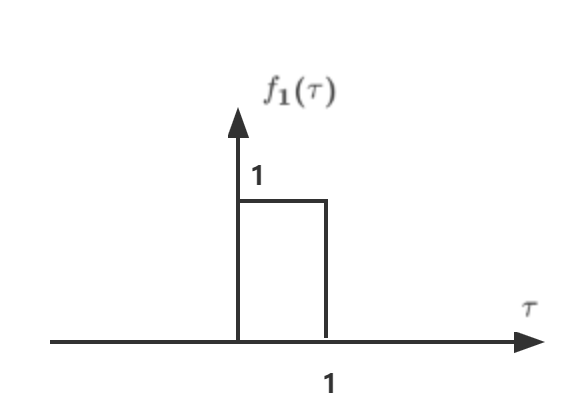
\includegraphics[width=5.5cm]{./figures/photo9.png}
			}
			\quad
			\subfigure[]{
			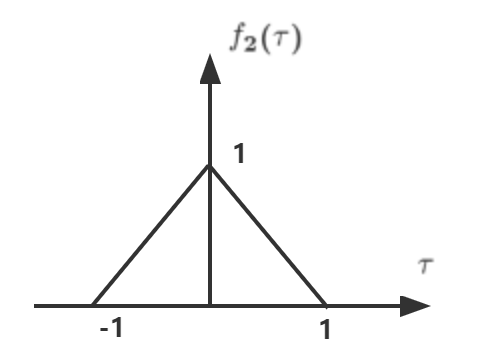
\includegraphics[width=5.5cm]{./figures/photo10.png}
			}
			\quad
			\subfigure[]{
			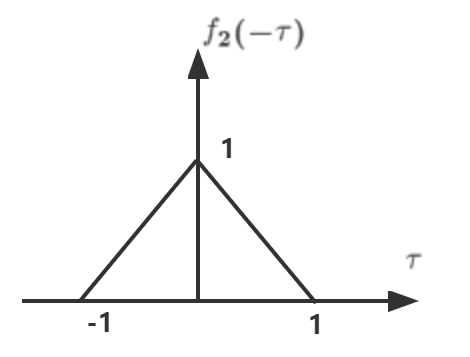
\includegraphics[width=5.5cm]{./figures/photo11.png}
			}
			\quad
			\subfigure[]{
			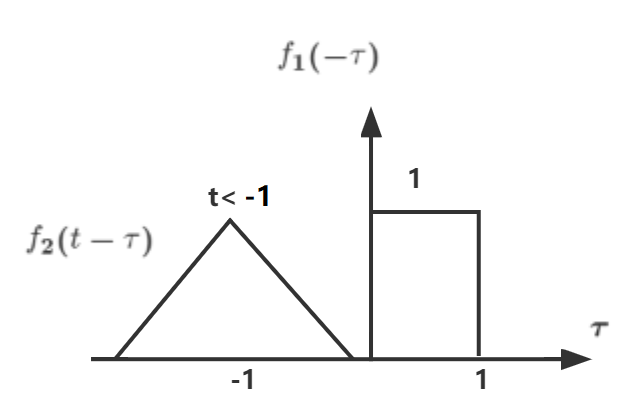
\includegraphics[width=5.5cm]{./figures/photo12.png}
			}
			\quad
			\subfigure[]{
			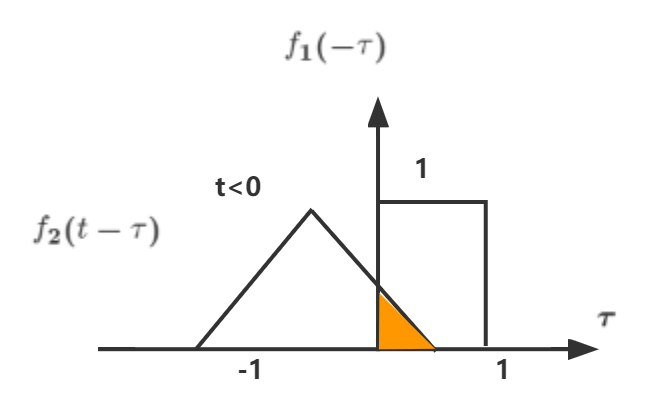
\includegraphics[width=5.5cm]{./figures/photo13.png}
			}
			\quad
			\subfigure[]{
			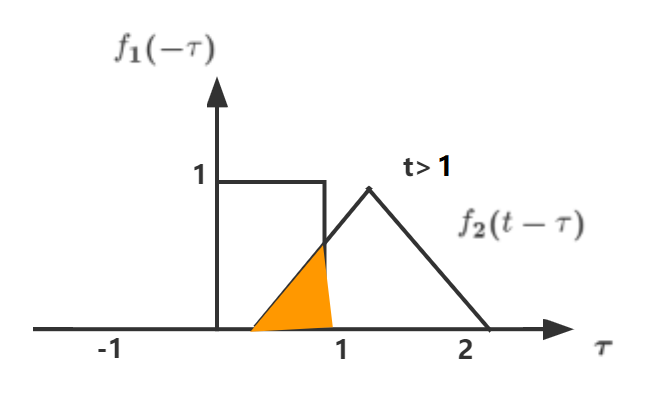
\includegraphics[width=5.5cm]{./figures/photo14.png}
			}
			\caption{卷积图解过程}
		\end{figure}
			(2)分三种情况讨论得:
			\[ y= \begin{cases}
			0.5t^2+t+0.5,\quad -1<t<0 \\
			-t^2+t+0.5,\quad 0<t<1 \\
			0.5t^2-2t+2,\quad 1<t<2\\
			\end{cases} \]
	\end{enumerate}
	\subsection{{\heiti\zihao{4}实验收获与心得}}
	通过本次实验对卷积积分和卷积和的概念进一步加深,熟悉卷积积分和卷积和的相关性质和求解方法,同时也学会利用Matlab 工具箱求解连续时间系统的冲激响应、阶跃响应,离散时间系统的单位样值响应,还掌握了有关信号时域的测量方法。
\end{document}